\documentclass[10pt,a4paper,notitlepage]{article}
\usepackage[utf8]{inputenc}
\usepackage{amsmath}
\usepackage{amsfonts}
\usepackage{amssymb}
\usepackage{fullpage}
\usepackage{lastpage}
\usepackage{fancyhdr}
\usepackage{fancyvrb}
\usepackage{graphicx}
\graphicspath{{./Graphics/}}
\usepackage{float}
\usepackage{nameref}
\usepackage[backend=bibtex,style=verbose-trad2]{biblatex}
\author{Jonah Gibbon}
\bibliography{References}


\pagestyle{fancy}
\fancyhf{}
\renewcommand{\headrulewidth}{0pt}
\cfoot{Page \thepage\ of \pageref{LastPage}}

\newcommand{\abs}[1]{\lvert#1\rvert}
\newcommand{\Z}{\mathbb{Z}}
\newcommand{\Q}{\mathbb{Q}}
\newcommand{\C}{\mathbb{C}}
\newcommand{\N}{\mathbb{N}}
\newcommand{\R}{\mathbb{R}}

\begin{document}
\section*{\centering \large Programming Task}
\nameref{subsec:Code 1.1} referenced page \pageref{subsec:Code 1.1} was used to compute the approximation $Y_{n}$ using the Euler and Runge-Kutta method.\footnote{Note that the functions \texttt{Euler} and \texttt{RK4} defined in Code 1.1 will be used throughout the project, and so their definitions will not be included in any further code's referencing.} To test that the program was running properly, \nameref{subsec:Code 1.2} referenced page \pageref{subsec:Code 1.2} produced Figure 1, a plot of both solutions $Y_{n}$ with the exact solution $y(x)$ superimposed.  $Y_{n}$ was calculated over the interval $[0,1]$ with $h=0.1$.\\
\begin{figure}[H]
\begin{center}
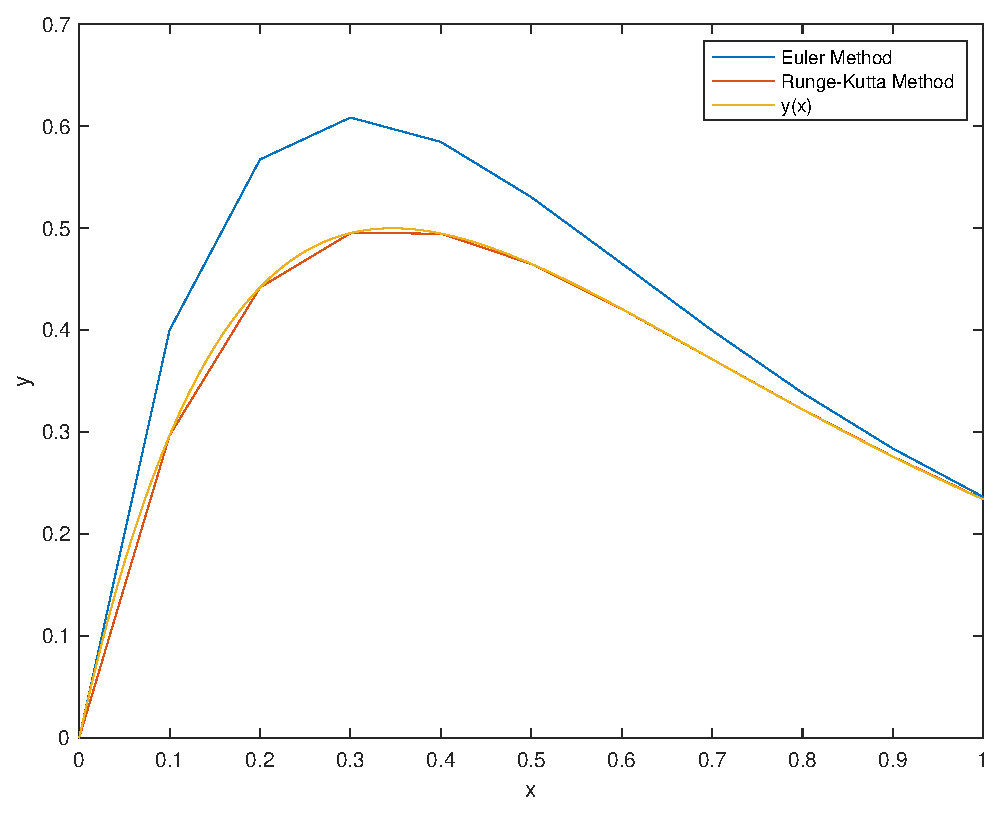
\includegraphics[width=10cm]{Image_1_1}
\caption{Plot of $Y_{n}$ using Euler and RK4 methods with exact solution}
\end{center}
\end{figure}
\section*{\centering \large Question 1}
Code 1.1 was used to produce Tables 1-7 with the appropriate changes to $h$. 
\begin{table}[H]
\begin{center}
\begin{tabular}{|c|c|c|c|c|} 
\hline
$x_{n}$&$Y_{n}$&$y(x_{n})$&$E_{n}$&$E_{n}/E_{n-1}$\\ \hline
0 & 0 & 0 & 0 & 0\\  2.0 & 8.0 & 0.03596 & 7.964 & $\infty$ \\  4.0 & -55.853 & 0.0006707 & -55.854 & -7.0133\\ 6.0 & 390.98 & 0.000012288 & 390.98 & -7.0\\ 8.0 & -2736.8 & 2.2507e-7 & -2736.8 & -7.0\\ 10.0 & 19158.0 & 4.1223e-9 & 19158.0 & -7.0\\ 12.0 & -134110.0 & 7.5503e-11 & -134110.0 & -7.0\\ \hline
\end{tabular}
\caption{Euler method for equation (5a) with $h=2$}
\end{center}
\end{table}
Observe in Table 1 that $\abs{E_{n}}\rightarrow \infty$, suggesting this approximation is unstable. The last column of Table 1 suggests the error grows 7 times larger with every step.  Therefore, for large $n$,  $\abs{E_{n}/E_{n-1}}=e^{\gamma h}$, and since $h=2$, we calculate $\gamma=\ln(7)/2$.\\

Below are the same approximations for $Y_{n}$ with different values of $h$. Parts of the data has been omitted. 

\begin{table}[H]
\parbox{.45\linewidth}{
\centering
\begin{tabular}{|c|c|c|c|} \hline
$x=n$ & $Y_{n}$ & $E_{n}$ & $E_{n}/E_{n-1}$\\ 
\hline 1.0 & 4.0 & 3.766 & $\infty$ \\ 2.0 & -11.459 & -11.495 & -3.0522\\ 3.0 & 34.449 & 34.444 & -2.9966\\ 4.0 & -103.34 & -103.34 & -3.0002 \\ $\vdots$ & $\vdots$ & $\vdots$ & $\vdots$ \\  11.0 & 226000.0 & 226000.0 & -3.0\\ 12.0 & -678000.0 & -678000.0 & -3.0\\ \hline \end{tabular}
\caption{$h=1.0$}
}
\hfill
\parbox{.45\linewidth}{
\centering
\begin{tabular}{ |c|c|c|c| }
\hline
$x=0.6n$ & $Y_{n}$ & $E_{n}$ & $E_{n}/E_{n-1}$\\ 
\hline
0.6 & 2.4 & 1.979 & $\infty$ \\ 1.2 & -2.6371 & -2.8021 & -1.4159\\ 1.8 & 3.9097 & 3.8566 & -1.3763\\ 2.4 & -5.408 & -5.4243 & -1.4065 \\ $\vdots$ & $\vdots$ & $\vdots$ & $\vdots$\\ 11.4 & 843.12 & 843.12 & -1.4\\ 12.0 & -1180.4 & -1180.4 & -1.4\\ \hline \end{tabular}
\caption{$h=0.6$}
}
\end{table}

\begin{table}[H]
\parbox{.45\linewidth}{
\centering
\begin{tabular}{|c|c|c|c|}
\hline
$x=0.5n$ & $Y_{n}$ & $E_{n}$ & $E_{n}/E_{n-1}$\\ 
\hline 0.5 & 2.0 & 1.5349 & $\infty$ \\ 1.0 & -1.2642 & -1.4983 & -0.97613\\ 1.5 & 1.5349 & 1.4403 & -0.9613\\ 2.0 & -1.4353 & -1.4713 & -1.0215\\ $\vdots$ & $\vdots$ & $\vdots$ & $\vdots$\\ 11.5 & 1.4621 & 1.4621 & -1.0\\ 12.0 & -1.4621 & -1.4621 & -1.0\\ \hline \end{tabular}

\caption{$h=0.5$}
}
\hfill
\parbox{.45\linewidth}{
\centering
\begin{tabular}{|c|c|c|c|}
\hline
$x=0.4n$ & $Y_{n}$ & $E_{n}$ & $E_{n}/E_{n-1}$\\ 
\hline
0.4 & 1.6 & 1.1051 & $\infty$ \\ 0.8 & -0.24107 & -0.56334 & -0.50975\\ 1.2 & 0.46768 & 0.3027 & -0.53733\\ 1.6 & -0.13546 & -0.21366 & -0.70584\\ $\vdots$ & $\vdots$ & $\vdots$ & $\vdots$\\ 11.6 & 5.6194e-7 & 5.6178e-7 & -0.5999\\ 12.0 & -3.3703e-7 & -3.3711e-7 & -0.60007\\ \hline \end{tabular}
\caption{$h=0.4$}
}
\end{table}

\begin{table}[H]
\parbox{.45\linewidth}{
\centering
\begin{tabular}{|c|c|c|c|}
\hline
$x=0.3n$ & $Y_{n}$ & $E_{n}$ & $E_{n}/E_{n-1}$\\ 
\hline
0.3 & 1.2 & 0.70477 & $\infty$ \\ 0.6 & 0.41857 & -0.0023786 & -0.003375\\ 0.9 & 0.27772 & 0.0017679 & -0.74328\\ 1.2 & 0.14282 & -0.022161 & -12.535\\ $\vdots$ & $\vdots$ & $\vdots$ & $\vdots$\\ 11.7 & 1.1023e-10 & -2.734e-11 & 0.54881\\ 12.0 & 6.0498e-11 & -1.5005e-11 & 0.54881\\ \hline \end{tabular}
\caption{$h=0.3$}
}
\hfill
\parbox{.45\linewidth}{
\centering
\begin{tabular}{|c|c|c|c|}
\hline
$x=0.2n$ & $Y_{n}$ & $E_{n}$ & $E_{n}/E_{n-1}$\\ 
\hline
0.2 & 0.8 & 0.35802 & $\infty$ \\ 0.4 & 0.69626 & 0.20139 & 0.56252\\ 0.6 & 0.49871 & 0.077762 & 0.38612\\ 0.8 & 0.3407 & 0.01843 & 0.237\\ $\vdots$ & $\vdots$ & $\vdots$ & $\vdots$\\ 11.8 & 9.5796e-11 & -1.6841e-11 & 0.67032\\ 12.0 & 6.4214e-11 & -1.1289e-11 & 0.67032\\ \hline \end{tabular}
\caption{$h=0.2$}
}
\end{table}
$E_{n}$ is still unstable in Tables 2 and 3 however it diverges slower than when $h=2$, meaning $0<\gamma<\ln(7)/2$. The global error has fixed magnitude in Table 4, suggesting that $\gamma$ is close to 0. In Tables 5-7 the solution is stable, i.e. $E_{n}$ tends to 0, so $\gamma<0$. We conclude that as $h$ decreases, the growth rate decreases, and that $Y_{n}$ is stable when the growth rate is negative, i.e. when $h$ is less than a certain value which is approximately 0.5.  Observe that in the last column of Table 7 the error ratio is larger than that in Table 6. This is due to the code dividing by a small number that cannot be stored to a high enough precision. 
\section*{\centering \large Question 2}
We can rewrite the difference equation as
\begin{equation}
Y_{n}=\left( 1-4h\right) Y_{n-1}+4h\left( e^{-2h}\right) ^{n}
\end{equation}
Expanding this, and using the fact that $Y_{0}=0$ gives
\begin{equation}
\begin{aligned}
Y_{n}&=4h\left(e^{-2h}\right)^{n-1}\sum_{r=0}^{n-1}\left(e^{2h}\left(1-4h\right)\right)^{r}\\
&=4h\left( e^{-2h}\right)^{n-1}\left(\frac{1-(1-4h)^{n}\left( e^{2h}\right) ^{n}}{1-\left( 1-4h\right)e^{2h}}\right)
\end{aligned}
\end{equation}
Instability occurs if the infinite sum diverges faster than the coefficient on the front converges to 0. The leading term in equation (2) is $4h(1-4h)^{n-1}$, so instability occurs when $h\geq 1/2$ since then $\abs{1-4h}>1$ and $Y_{n}\rightarrow \infty$. For large $n$ the error ratio is $\exp\left( \ln\left(\abs{1-4h}\right)\right)$, and so we conclude that the growth rate is $\ln\left(\abs{1-4h}\right)/h$. These conclusions are consistent with the values in Question 1.\\

If $x_{n}=nh$ remains fixed, we may write $h=x_{n}/n$. So $(1-4h)^{n}\rightarrow e^{-4x_{n}}$ and
\begin{equation}
\begin{aligned}
Y_{\infty}&=\lim_{h\rightarrow 0}4h\left( e^{-2x_{n}}\right) e^{2h}\left(\frac{1-e^{-2x_{n}}}{1-\left(1-4h\right)e^{2h}}\right)\\
&= \left(4e^{-2x_{n}}-4e^{-4x_{n}}\right)\lim_{h\rightarrow 0}\frac{h}{1-\left( 1-4h\right) e^{2h}}\\
&= \left( 4e^{-2 x_{n}}-4 e^{-4 x_{n}}\right) \lim _{h \rightarrow 0}\frac{1}{-2 e^{2 h}+4 e^{2 h}+8 h e^{2 h}}
\end{aligned}\\
\end{equation}
using l'hôpital's rule. The result follows.
\section*{\centering \large Question 3}
Code 1.1 was used to produce Tables 8-9 with the changes that $h=0.4$ and the interval being integrated over as $[0,6]$.
\begin{table}[H]
\centering
\begin{tabular}{|c|c|c|c|c|}
\hline
$x_{n}$&$Y_{n}$&$y(x_{n})$&$E_{n}$&$E_{n}/E_{n-1}$\\ \hline
0 & 0 & 0 & 0 & 0\\ 0.4 & 1.6 & 0.49486 & 1.1051 & $\infty$ \\ 0.8 & -0.24107 & 0.32227 & -0.56334 & -0.50975\\ 1.2 & 0.46768 & 0.16498 & 0.3027 & -0.53733\\ 1.6 & -0.13546 & 0.078201 & -0.21366 & -0.70584\\ 2.0 & 0.14649 & 0.03596 & 0.11053 & -0.51734\\ 2.4 & -0.058592 & 0.016324 & -0.074916 & -0.67776\\ 2.8 & 0.048323 & 0.0073684 & 0.040954 & -0.54667\\ 3.2 & -0.023077 & 0.0033176 & -0.026395 & -0.64449\\ 3.6 & 0.016505 & 0.0014921 & 0.015013 & -0.56878\\ 4.0 & -0.0087083 & 0.0006707 & -0.009379 & -0.62474\\ 4.4 & 0.0057617 & 0.00030142 & 0.0054603 & -0.58218\\ 4.8 & -0.0032159 & 0.00013545 & -0.0033513 & -0.61376\\ 5.2 & 0.0020379 & 0.000060863 & 0.001977 & -0.58992\\ 5.6 & -0.001174 & 0.000027348 & -0.0012014 & -0.60768\\ 6.0 & 0.0007263 & 0.000012288 & 0.00071401 & -0.59432\\ \hline \end{tabular}
\caption{Euler method to solve equation (5a) with $h=0.4$}
\end{table}
\begin{table}[H]
\centering
\begin{tabular}{|c|c|c|c|c|}
\hline
$x_{n}$&$Y_{n}$&$y(x_{n})$&$E_{n}$&$E_{n}/E_{n-1}$\\ \hline
0 & 0 & 0 & 0 & 0\\ 0.4 & 0.39989 & 0.49486 & -0.094973 & $-\infty$ \\ 0.8 & 0.28781 & 0.32227 & -0.034455 & 0.36279\\ 1.2 & 0.15856 & 0.16498 & -0.0064148 & 0.18618\\ 1.6 & 0.079152 & 0.078201 & 0.00095115 & -0.14827\\ 2.0 & 0.037703 & 0.03596 & 0.0017429 & 1.8325\\ 2.4 & 0.017519 & 0.016324 & 0.0011952 & 0.68574\\ 2.8 & 0.0080282 & 0.0073684 & 0.00065983 & 0.55207\\ 3.2 & 0.0036496 & 0.0033176 & 0.00033198 & 0.50313\\ 3.6 & 0.0016513 & 0.0014921 & 0.00015923 & 0.47964\\ 4.0 & 0.00074506 & 0.0006707 & 0.000074362 & 0.467\\ 4.4 & 0.00033561 & 0.00030142 & 0.000034193 & 0.45982\\ 4.8 & 0.00015103 & 0.00013545 & 0.000015579 & 0.45561\\ 5.2 & 0.000067922 & 0.000060863 & 7.0587e-6 & 0.45311\\ 5.6 & 0.000030536 & 0.000027348 & 3.1877e-6 & 0.4516\\ 6.0 & 0.000013725 & 0.000012288 & 1.4367e-6 & 0.4507\\ \hline \end{tabular}
\caption{Runge-Kutta method to solve equation (5a) with $h=0.4$}
\end{table}
It can be seen that the error in the Runge-Kutta decreases at a faster rate than the Euler method, and this is better presented in Figure 2 below, produced by Code 1.2. Both numerical solutions have the same long time behaviour as the exact solution; both methods are stable.
\begin{figure}[H]
\begin{center}
\includegraphics[width=10cm]{Image_2_1}
\caption{Plot of $Y_{n}$ using Euler and RK4 methods with exact solution where $h=0.4$}
\end{center}
\end{figure}
\pagebreak
\section*{\centering \large Question 4}

\nameref{subsec:Code 4.1} referenced page \pageref{subsec:Code 4.1} produced Table 10 and Figures 3-4 below. 
\begin{table}[H]
\centering
\begin{tabular}{|c|c|c|}
\hline $h$ & $E_{n}$ using Euler & $E_{n}$ using RK4 \\ \hline 1.6 & 6.3218 & -51.339\\ 0.8 & -6.4721 & -4.2435\\ 0.4 & -0.21366 & 0.00095115\\ 0.2 & -0.0088704 & 0.00010423\\ 0.1 & -0.004174 & 5.5117e-6\\ 0.05 & -0.00195 & 3.1351e-7\\ 0.025 & -0.00093479 & 1.8658e-8\\ 0.0125 & -0.00045677 & 1.1374e-9\\ 0.00625 & -0.00022566 & 7.02e-11\\ 0.003125 & -0.00011215 & 4.3599e-12\\ 0.0015625 & -0.0000559 & 2.7156e-13\\ 0.00078125 & -0.000027907 & 1.6889e-14\\ 0.00039062 & -0.000013943 & 1.138e-15\\ 0.00019531 & -6.9686e-6 & 3.1919e-16\\ 0.000097656 & -3.4836e-6 & -6.9389e-17\\ 0.000048828 & -1.7416e-6 & 2.7756e-16\\ \hline \end{tabular}
\caption{$E_{n}$ at $x_{n}=1.6$ using Euler and RK4 methods for various $h$}
\end{table}
\begin{figure}[H]
\begin{center}
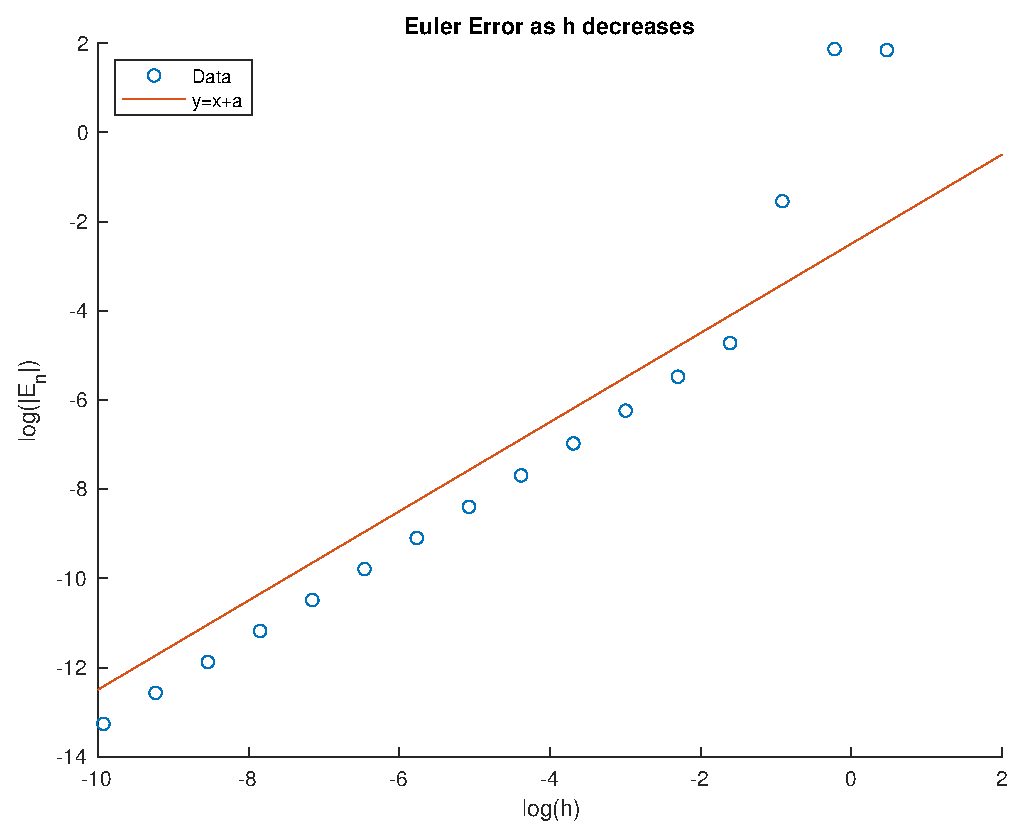
\includegraphics[width=12cm]{Image_4_1}
\caption{$\log(|E_{n}|)$ against $\log(h)$ using the Euler method}
\end{center}
\end{figure}
\begin{figure}[H]
\begin{center}
\includegraphics[width=12cm]{Image_4_2}
\caption{$\log(|E_{n}|)$ against $\log(h)$ using the RK4 method}
\end{center}
\end{figure}
Both methods bear out their theoretical orders of accuracy. If a general method is $n$-th order accurate, then we may write $E(h)=Ch^{n}$ where $C$ is some constant and $E(h)$ is the error in approximating a given point with step size $h$.  Therefore $\log(E(h))=n\log(h)+\log(C)$, so plotting $\log(E(h))$ against $\log(h)$ would give a straight line with gradient $n$. \nameref{subsec:Code 4.1} superimposes the straight lines $x+a$ and $4x+b$ for some constants $a$ and $b$ to illustrate this point for the Euler and Runge Kutta methods respectively. Note that the data points in Figure 4 tend upwards as $\log\left(h\right)$ gets small. This is due to the program not being able to store $h^{4}$ to a high enough order of accuracy and so when dividing by them there is a large possible error.

\section*{\centering \large Question 5}
\nameref{subsec:Code 1.1} was used to produce the data in Table 11 with the appropriate changes to the interval integrated over, $h$, $f(x,y)$, and the exact solution $y(x)$.
\begin{table}[H]
\centering
\begin{tabular}{|c|c|c|c|c|} \hline $x=0.2n$ & $Y_{n}$ & $y(x)$ & $E_{n}$ & $E_{n}/E_{n-1}$\\ \hline 0 & 1.0 & 1.0 & 0 & 0\\ 0.001 & 0.999 & 0.999 & -4.9983e-7 & $-\infty$ \\ 0.002 & 0.998 & 0.998 & -1.0012e-6 & 2.003\\ 0.003 & 0.997 & 0.997 & -1.504e-6 & 1.5023\\ 0.004 & 0.99601 & 0.99601 & -2.0084e-6 & 1.3353\\ 
$\vdots$&$\vdots$&$\vdots$&$\vdots$&$\vdots$\\
9.998 & -2.1556e+13  & 4.5491e-05 & -2.1556e+13  & 1.004\\
9.999 & -2.1642e+13   &4.5445e-05  &-2.1642e+13      &  1.004\\
           10  &-2.1728e+13 &    4.54e-05 & -2.1728e+13     &   1.004\\ \hline \end{tabular}
\caption{Euler Method used to solve Question 5}
\end{table}
It can be seen that the error ratio is just greater than 1,  suggesting that this approximation does grow exponentially.  Following a similar method to Question 2, expanding the Euler difference equation and summing the geometric series gives
\begin{equation}
Y_{n}=\left( 1+4h\right) ^{n} -5h \left( 1+4h \right) ^{n-1} \frac{1-e^{-hn}\left( 1+4h\right) ^{-n}}{1-e^{-h}\left( 1+4h \right)^{-1}}
\end{equation}
The dominant term in this equation is $(1+4h)^{n}$, so for large $n,  E_{n}\approx (1+4h)^{n}$. Therefore for any $h>0$ the error cannot be suppressed using the Euler method.  Expanding the Runge-Kutta difference equation gives
\begin{equation}
\begin{aligned}
Y_{n+1} &= \left(1+4h\right)Y_{n}-5he^{-x_{n}}+O(h^{2})Y_{n}+O(h^{2})e^{-x_{n}}\\
&= Y_{n} + hf\left( x_{n},Y_{n}\right) +O(h^{2})Y_{n}+O(h^{2})e^{-x_{n}}
\end{aligned}
\end{equation}
As $h\rightarrow 0$, the difference equation above tends to the Euler difference equation, so both methods would give the same solution. Therefore the error wouldn't be suppressed with a small $h$ using the Runge-Kutta method.

\section*{\centering \large Question 6}
When $p=0$ the original differential equation becomes $y''(x)=0$ so $y=ax+b$. Imposing initial conditions gives the trivial solution $y=0$.   Differentiating the general solution gives 
\begin{equation}
\frac{dy}{dx}=A\sin(p(1+x)^{-1}-\phi)-Ap(1+x)^{-1}\cos(p(1+x)^{-1}-\phi)
\end{equation} 
so imposing conditions (15) in the booklet gives
\begin{equation}
\begin{aligned}
A\sin(p-\phi) &= 0\\
-Ap\cos\left( p-\phi\right) &= 1
\end{aligned}
\end{equation}
This implies that $p-\phi=\pi k$ where $k\in \Z$, and $A=(-1)^{k-1}/p$ (It is assumed $p\neq 0$ otherwise the formula given would not hold).  So the particular solution is
\begin{equation}
\begin{aligned}
y &= \frac{(-1)^{k-1}}{p}\left(1+x\right) \sin \left( \frac{p}{1+x}-p+k\pi\right)\\
&= \frac{1}{p}\left(1+x\right) \sin \left( \frac{px}{1+x}\right)
\end{aligned}
\end{equation}
Imposing the condition $y(1)=0$ means that $\sin\left(p/2\right)=0$. Hence the smallest (positive) eigenvalue is $p=2\pi$ and all eigenvalues are of the form $p_{n}=2\pi n$ where $n\in\Z$.  The corresponding eigenfunctions are
\begin{equation}
y_{n}=A\left(1+x\right) \sin \left(\frac{2\pi nx}{1+x}\right)
\end{equation}
where $A$ is an arbitrary constant.
\section*{\centering \large Programming Task}
\nameref{subsec:Code 7.1} referenced page \pageref{subsec:Code 7.1} was used to calculate the analytic solution with $x_{0}=0, y_{0}=0, z_{0}=1, x_{n}=\pi/2, h=\pi/100, p=1, \alpha=0$. The exact solution to this problem is $\sin\left(x\right)$, so the expected outcome is $Y_{n}=1$. 
\begin{table}[H]
\centering
\begin{tabular}{|c|c|c|} \hline$x_{n}$&$Y_{n}$&$Y'_{n}$\\ \hline 0 & 0 & 1.0\\ 0.031416 & 0.031411 & 0.99951\\ 0.062832 & 0.062791 & 0.99803\\ $\vdots$&$\vdots$&$\vdots$ \\ 1.5394 & 0.99951 & 0.031411\\ 1.5708 & 1.0 & 1.2746e-8\\ \hline\end{tabular}
\caption{Test data for Programming Task}
\end{table}
This is correct, so the programme works.\footnote{The functions $\mathtt{RK4Vector}$ and $\mathtt{F}$ defined in Code 7.1 will be used throughout the rest of this project. They will not be defined in further code.}

\section*{\centering \large Question 7}
\nameref{subsec:Code 7.2} referenced page \pageref{subsec:Code 7.2} is a modification of \nameref{subsec:Code 7.1} and was used to produce the data in Tables 13-14. 
\begin{table}[H]
\centering
\begin{tabular}{|c|c|c|c|c|c|} \hline $h$&$Y_{n}(1)$&$Y'_{n}(1)$&$y(1)$&$E_{n}$&$E_{n}/h^{4}$ \\ \hline 0.1 & 0.047118 & -0.47125 & 0.04704 & 0.000078172 & 0.78172\\ 0.05 & 0.047047 & -0.47146 & 0.04704 & 6.8166e-6 & 1.0906\\ 0.025 & 0.04704 & -0.47148 & 0.04704 & 4.6574e-7 & 1.1923\\ 0.0125 & 0.04704 & -0.47148 & 0.04704 & 2.9972e-8 & 1.2277\\ 0.00625 & 0.04704 & -0.47148 & 0.04704 & 1.8941e-9 & 1.2413\\ 0.003125 & 0.04704 & -0.47148 & 0.04704 & 1.1893e-10 & 1.2471\\ 0.0015625 & 0.04704 & -0.47148 & 0.04704 & 7.449e-12 & 1.2497\\ 0.00078125 & 0.04704 & -0.47148 & 0.04704 & 4.6559e-13 & 1.2498\\ 0.00039062 & 0.04704 & -0.47148 & 0.04704 & 2.8963e-14 & 1.2439\\ 0.00019531 & 0.04704 & -0.47148 & 0.04704 & 1.5335e-15 & 1.0538\\ 0.000097656 & 0.04704 & -0.47148 & 0.04704 & -3.2613e-16 & -3.5858\\ 0.000048828 & 0.04704 & -0.47148 & 0.04704 & 2.8449e-16 & 50.049\\ 0.000024414 & 0.04704 & -0.47148 & 0.04704 & -7.6328e-17 & -214.84
 \\ \hline \end{tabular}
\caption{RK4 approximation of 2nd order ODE with $p=6$}
\label{tab:P=6}
\end{table}

\begin{table}[H]
\centering
\begin{tabular}{|c|c|c|c|c|c|} \hline $h$&$Y_{n}(1)$&$Y'_{n}(1)$&$y(1)$&$E_{n}$&$E_{n}/h^{4}$ \\ \hline 0.1 & -0.09995 & -0.51797 & -0.10022 & 0.00027401 & 2.7401\\ 0.05 & -0.10021 & -0.51833 & -0.10022 & 0.000018526 & 2.9641\\ 0.025 & -0.10022 & -0.51834 & -0.10022 & 1.1413e-6 & 2.9218\\ 0.0125 & -0.10022 & -0.51834 & -0.10022 & 6.9846e-8 & 2.8609\\ 0.00625 & -0.10022 & -0.51834 & -0.10022 & 4.3039e-9 & 2.8206\\ 0.003125 & -0.10022 & -0.51834 & -0.10022 & 2.6684e-10 & 2.798\\ 0.0015625 & -0.10022 & -0.51834 & -0.10022 & 1.6606e-11 & 2.7861\\ 0.00078125 & -0.10022 & -0.51834 & -0.10022 & 1.0353e-12 & 2.7791\\ 0.00039062 & -0.10022 & -0.51834 & -0.10022 & 6.4893e-14 & 2.7871\\ 0.00019531 & -0.10022 & -0.51834 & -0.10022 & 3.9413e-15 & 2.7084\\ 0.000097656 & -0.10022 & -0.51834 & -0.10022 & 4.8572e-16 & 5.3406\\ 0.000048828 & -0.10022 & -0.51834 & -0.10022 & 1.471e-15 & 258.79\\ 0.000024414 & -0.10022 & -0.51834 & -0.10022 & 1.9429e-15 & 5468.8\\ \hline \end{tabular}
\caption{RK4 approximation of 2nd order ODE with $p=7$}
\label{tab:P=7}
\end{table}
The error in this program behaves as expected, since plotting $E_{n}$ against $h^{4}$ gives a constant,  implying that this method is indeed 4th order convergent. In both cases this column grows out of control as $h$ grows small. This can be explained by the fact that $h^{4}$ is very small and MATLAB cannot store it to a high enough precision. Therefore dividing by it gives a large possibility for error. 
\section*{\centering \large Programming Task}
\nameref{subsec:Code 8.1} referenced page \pageref{subsec:Code 8.1} was used to produce the test data in Table 15.  The function $g(p)=x^{2}-3$ with starting interval $[0,3]$, and so the root being searched for is $\sqrt{3}$.  Clearly the code works.
\begin{table}[H]
\centering
\begin{tabular}{|c|c|c|}
\hline 
Iteration $n$ & $P_{n}$ & $g(P_{n})$ \\ 
\hline 
0 & 0 & -3.0\\ 1.0 & 1.0 & -2.0\\ 2.0 & 1.5 & -0.75\\ 3.0 & 1.6666667 & -0.22222222\\ $\vdots$&$\vdots$&$\vdots$\\ 12.0 & 1.7320503 & -0.0000016436546\\ 13.0 & 1.7320507 & -0.00000044041601\\
\hline 
\end{tabular} 
\caption{Test data for bisection method}
\end{table}
\section*{\centering \large Question 8}
Code 8.1 referenced page \pageref{subsec:Code 8.1} produced the iterates in Table 16 with the values $h=7.3\times 10^{-7}$ and $\epsilon=0.001$. It has the alteration that $\mathtt{LowerP}=6, \mathtt{UpperP=7}$ at the start, and that the function $g$ is instead defined as

\begin{verbatim}
function answer=g(x)
    answer=RK4Vector(0,1,0,1,0.001,x,4);
    answer=answer(end,2);
end
\end{verbatim}

\begin{table}[H]
\centering
\begin{tabular}{|c|c|c|}
\hline Iteration $n$& $P_{n}$ & $g(P_{n})$\\ \hline
1 & 6.319426827431968 & -0.005734624021197 \\
2 & 6.284717102857235 & -2.437334079506857e-04 \\
3 & 6.283249472007579 & -1.021204360527814e-05 \\
4 & 6.283187993946834 & -4.276104517038359e-07 \\
\hline \end{tabular}
\caption{Approximation of smallest eigenvalue with $\alpha=4$}
\end{table}

In order to justify the choice of $\epsilon$, we must first approximate the gradient $g'(p_{*})$ where $p_{*}$ is the eigenvalue. Assuming that $g''(p)$ is small in the interval $[6,7]$, $g'(p_{*})\approx g(7)-g(6)=-0.14726$, and so in order for the error in the approximation to be less than $\pm 5\times 10^{-6}$, it is sufficient to choose $\epsilon\leq 5\times 10^{-6} \times 0.14726=7.3\times 10^{-7}$. This works on the assumption that $g(p)$ is evaluated perfectly at each value of $p$. \\

Suppose we iterated one step of the false-position method over the interval $[a,b]$, however the value $g(a)$ was perturbed as $g(a)+\delta_{1}$, and $g(b)$ as $g(b)+\delta_{2}$. As long as $\left( g(a)+\delta_{1} \right)\left( g(b)+\delta_{2}\right) < 0$, the iteration will move closer towards the root. Therefore the error approximating $g(p)$ shouldn't change the signs of any values. Assuming that $g(p)>7.3\times 10^{-7}$, otherwise the code would terminate, we require the error in approximating $g(p)$ to be less than $7.3\times 10^{-7}$.  \\

To find a suitable $h$, we must first show $\abs{y(x)}\leq x$ for all $x\geq 0$. We argue that $\abs{y'(x_{*})}\leq 1$ for any root $y(x_{*})=0$ using equation 13a in the booklet. We may visualise this equation as modelling a particle with a restoring force causing it to oscillate. Since this restoring force decreases with time $x$, it doesn't make sense for this particle to return to 0 faster than it left. By setting $y'(0)=1$, we ensure that $\abs{y'(x_{*})}\leq 1$, and so $\abs{y(x)}\leq x$ for all $x\geq 0$. Note this is true for all $\alpha\geq 0$.\\

Finding a $h_{0}$ such that $-1<g(p)<1$ means the error  is at most 2. Since the error in approximating $g(p)$ behaves as $O\left(h^{4}\right)$, we find a $k$ such that $2\times k^{4}\leq 7.3\times 10^{-7}$ or that $k\leq 0.0245$.  Therefore we pick our final $h$ as $h_{0}k$. Using the data in Tables \ref{tab:P=6}-\ref{tab:P=7}, we choose $h_{0}=0.1$ and $k= 0.01$, and so $h=0.001$ is sufficient. (The absolute error in Table 16 is $2.686\times 10^{-6}$.)\\ 


\section*{\centering \large Question 9}
\nameref{subsec:Code 9.1} referenced page \pageref{subsec:Code 9.1} was used to produce Table \ref{5Eigenvals} and Figures \ref{FFigure9}-\ref{LFigure9}.
\begin{table}[H]
\centering
\begin{tabular}{|c|}
\hline Eigenvalues\\ \hline 10.35892178053953\\ 21.2639307728608\\ 32.10538539075143\\ 42.91933654669045\\ 53.71911187891973\\ \hline \end{tabular}
\caption{Smallest eigenvalues with $\alpha=8$}\label{5Eigenvals}
\end{table}
These eigenvalues are the smallest possible. Code 9.1 searches upwards to find an interval of length one that straddles the root $g(p)=0$. Once it has found these intervals, it clarifies that $-1<g(p)<1$ to ensure the initial error is less than 2. To find a suitable $\epsilon$ it approximates the smallest value of $\abs{g'(p_{*})}$ using the method in Question 8. This $\epsilon$ is calculated as $1.08\times 10^{-7}$, so we choose a $k$ such that $2\times k^{4}\leq 1.08\times 10^{-7}$, or $k=0.01$. Therefore $h=0.001$ is sufficient for the eigenvalues to have an error less than $\pm5\times 10^{-6}$.
\begin{figure}[H]
\begin{center}
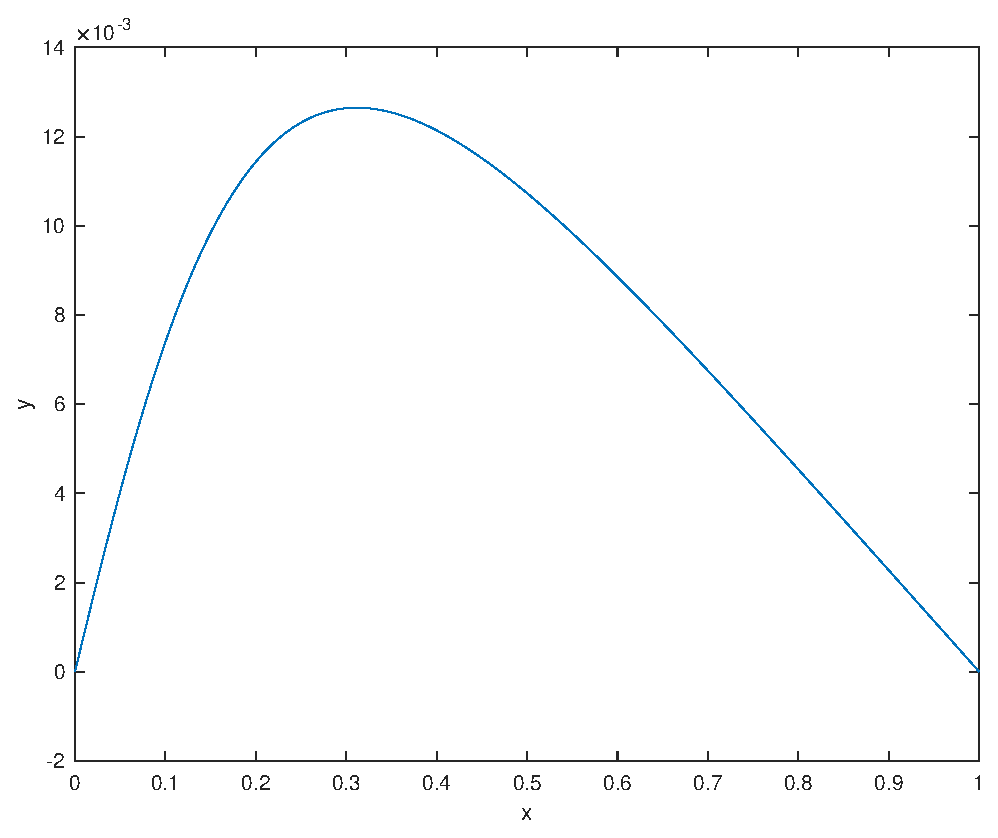
\includegraphics[width=10cm]{Image_9_1}
\caption{Normalised $y(x)$ using smallest eigenvalue $p=10.4$}\label{FFigure9}
\end{center}
\end{figure}
\begin{figure}[H]
\begin{center}
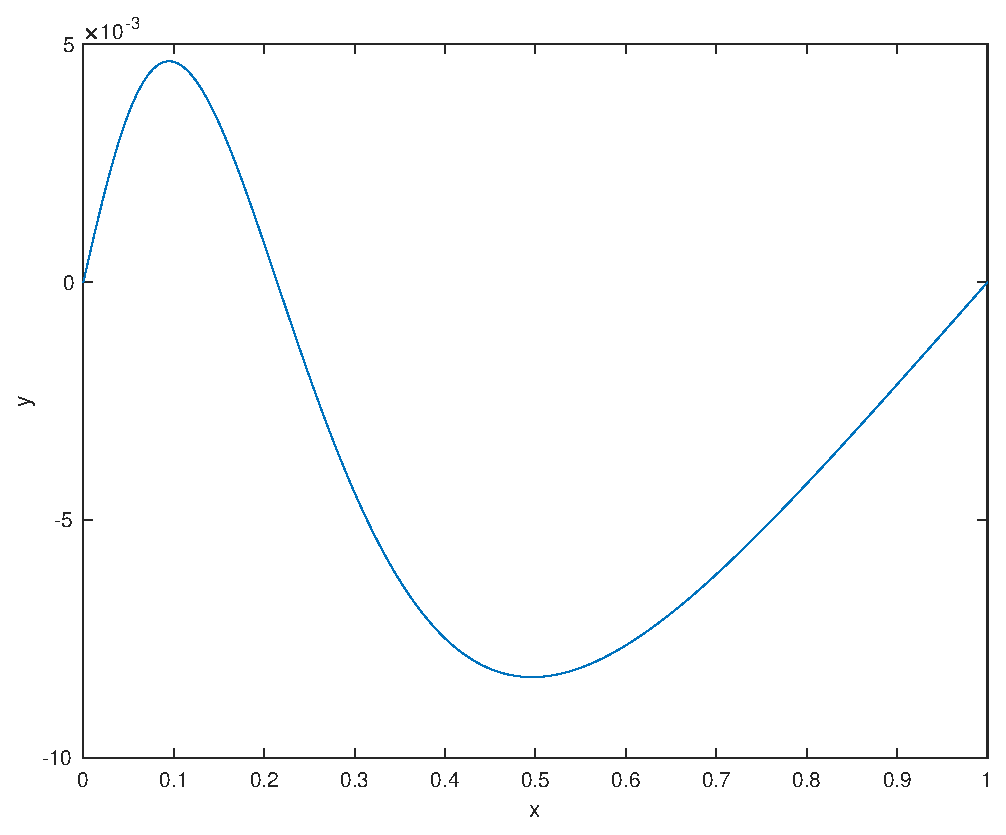
\includegraphics[width=10cm]{Image_9_2}
\caption{Normalised $y(x)$ using 2nd smallest eigenvalue $p=21.3$}
\end{center}
\end{figure}
\begin{figure}[H]
\begin{center}
\includegraphics[width=10cm]{Image_9_3}
\caption{Normalised $y(x)$ using 3rd smallest eigenvalue $p=32.1$}
\end{center}
\end{figure}
\begin{figure}[H]
\begin{center}
\includegraphics[width=10cm]{Image_9_4}
\caption{Normalised $y(x)$ using 4th smallest eigenvalue $p=42.9$}
\end{center}
\end{figure}
\begin{figure}[H]
\begin{center}
\includegraphics[width=10cm]{Image_9_5}
\caption{Normalised $y(x)$ using 5th smallest eigenvalue $p=53.7$}\label{LFigure9}
\end{center}
\end{figure}
In all figures there appears to be greater oscillation as $x$ increases, which makes sense since the mass distribution $\mu (x)$ decreases. It can also be seen that $\abs{y'(x_{*})}$ decreases as the roots $x_{*}$ increase, hypothesised is Question 8. The normalisation condition $\int_{0}^{1}\left(y'(x)\right)^{2}dx=1$ means the figures are easier to compare since the gradients are in proportion.





\pagebreak
\section*{\centering \large Code}
\subsection*{\centering\normalsize Code 1.1}\label{subsec:Code 1.1}
\begin{verbatim}
%Formats the output
format short g
digits(5)
data=Euler(0,1,0,0.1)
%Creates Latex code for the table
latex(sym(vpa(data)))
data=RK4(0,1,0,0.1)
latex(sym(vpa(data)))

function data = Euler(x_0,x_n,y_0,h)
%Creates a table to be filled
    data=zeros(ceil((x_n-x_0)/h)+1,5);
    data(1,:)=[x_0,y_0,y(x_0),y_0-y(x_0),0];
    counter=2;
%Iterates through the rows filling them
    while counter<=ceil((x_n-x_0)/h)+1
        data(counter,:)=[(counter-1)*h+x_0,...
            data(counter-1,2)+h*f((counter-2)*h+x_0,data(counter-1,2)),...
            y((counter-1)*h+x_0),...
            data(counter-1,2)+h*f((counter-2)*h+x_0,data(counter-1,2))-...
            y((counter-1)*h+x_0),...
            (data(counter-1,2)+h*f((counter-2)*h+x_0,data(counter-1,2))-...
            y((counter-1)*h+x_0))/data(counter-1,4)];
        counter=counter+1;
    end
end
function data = RK4(x_0,x_n,y_0,h)
%Follows a similar idea to the Euler function
    data=zeros(ceil((x_n-x_0)/h)+1,5);
    data(1,:)=[x_0,y_0,y(x_0),y_0-y(x_0),0];
    counter=2;
    while counter<=ceil((x_n-x_0)/h)+1
        k1=h*f((counter-2)*h+x_0,data(counter-1,2));
        k2=h*f((counter-2+1/2)*h+x_0,data(counter-1,2)+1/2*k1);
        k3=h*f((counter-2+1/2)*h+x_0,data(counter-1,2)+1/2*k2);
        k4=h*f((counter-2+1)*h+x_0,data(counter-1,2)+k3);
        data(counter,:)=[(counter-1)*h+x_0,...
            data(counter-1,2)+1/6*(k1+2*k2+2*k3+k4),...
            y((counter-1)*h+x_0),...
            data(counter-1,2)+1/6*(k1+2*k2+2*k3+k4)-y((counter-1)*h+x_0),...
            (data(counter-1,2)+1/6*(k1+2*k2+2*k3+k4)-y((counter-1)*h+x_0))/...
            data(counter-1,4)];
        counter=counter+1;
    end
end
%These two functions were created to stop repeatedly defining them
function z = f(x,y)
    z = -4*y+4*exp(-2*x);
end
function z = y(x)
    z= -2*exp(-4*x)+2*exp(-2*x);
end
\end{verbatim}
\pagebreak
\subsection*{\centering\normalsize Code 1.2} \label{subsec:Code 1.2}
\begin{verbatim}
data=Euler(0,1,0,0.1);
plot(data(:,1),data(:,2))
hold on
data=RK4(0,1,0,0.1);
plot(data(:,1),data(:,2))
plot(linspace(0,1),y(linspace(0,1)))
%Adds labels and saves the image
legend({'Euler Method','Runge-Kutta Method','y(x)'},'location',...
    'northeast')
xlabel('x')
ylabel('y')
print('Image_1_1','-depsc')
\end{verbatim}
\pagebreak
\subsection*{\centering\normalsize Code 4.1} \label{subsec:Code 4.1}
\begin{verbatim}
k=0;
Error=zeros(16,3);
while k<=15
    h=1.6/(2^k);
    data=Euler(0,1.6,0,h);
    Error(k+1,:)=[h,data(end,4),0];
    data=RK4(0,1.6,0,h);
    Error(k+1,3)=data(end,4);
    k=k+1;
end
digits(5)
disp(Error)
latex(sym(vpa(Error)))
logError=log(abs(Error));
meanError=mean(logError);

scatter(logError(:,1),logError(:,2))
hold on
x=xlim;
plot(linspace(x(1),x(2)),linspace(x(1),x(2))+meanError(2)-...
    meanError(1))
% Adds labels and saves the image
legend({'Data','y=x+a'},'location',...
    'northwest')
title('Euler Error as h decreases')
xlabel('log(h)')
ylabel('log(|E_{n}|)')
print('Image_4_1','-depsc')

figure
scatter(logError(:,1),logError(:,3))
hold on
x=xlim;
plot(linspace(x(1),x(2)),4*linspace(x(1),x(2))+meanError(3)-...
    4*meanError(1))
%Adds labels and saves the image
legend({'Data','y=4x+b'},'location',...
    'northwest')
title('Runge-Kutta Error as h decreases')
xlabel('log(h)')
ylabel('log(|E_{n}|)')
print('Image_4_2','-depsc')
\end{verbatim}
\pagebreak
\subsection*{\centering \normalsize Code 7.1}\label{subsec:Code 7.1}
\begin{verbatim}
data=RK4Vector(0,pi/2,0,1,pi/100,1,0)
latex(sym(vpa(data)))

function Solution = RK4Vector(x_0,x_n,y_0,z_0,h,p,a)
%Creates the table of iterates
X=zeros(ceil(x_n/h)+1,1);
Y=zeros(ceil(x_n/h)+1,2);
Y(1,:)=[y_0,z_0];
X(1)=x_0;
counter=2;

%This fills the table using the Runge-Kutta method
while counter<=ceil((x_n-x_0)/h)+1
    X(counter)=(counter-1)*h;
    K1=h*F(X(counter-1),Y(counter-1,:),p,a);
    K2=h*F(X(counter-1)+h*1/2,Y(counter-1,:)+K1/2,p,a);
    K3=h*F(X(counter-1)+h*1/2,Y(counter-1,:)+K2/2,p,a);
    K4=h*F(X(counter-1)+h,Y(counter-1,:)+K3,p,a);
    Y(counter,:)=Y(counter-1,:)+(K1+2*K2+2*K3+K4)/6;
    counter=counter+1;
end
Solution=[X,Y];
end

%This is f(X,Y)
function out = F(x,Y,p,a)
    out=zeros(1,2);
    %f_1
    out(1)=Y(2);
    %f_2
    out(2)=-p^2*(1+x)^(-a)*Y(1);
end
\end{verbatim}
\pagebreak
\subsection*{\centering \normalsize Code 7.2}\label{subsec:Code 7.2}
\begin{verbatim}
format long
p=6;
a=4;
k=0;
data=zeros(13,6);
while k<=12
    h=0.1/(2^k);
    data(k+1,1)=h;
    Matrix=RK4Vector(0,1,0,1,h,p,a);
    data(k+1,2)=Matrix(end,2);
    data(k+1,3)=Matrix(end,3);
    data(k+1,4)=y(1,p);
    data(k+1,5)=Matrix(end,2)-y(1,p);
    data(k+1,6)=data(k+1,5)/h^4;
    k=k+1;
end
data
digits(5)
latex(sym(vpa(data)))

function output = y(x,p)
output= (1/p)*(1+x)*sin(p-p/(1+x));
end
\end{verbatim}
\pagebreak
\subsection*{\centering \normalsize Code 8.1}\label{subsec:Code 8.1}
\begin{verbatim}
format long
LowerP=0;
UpperP=3;
epsilon=7.3*10^(-7);
%This records all the iterates
iterates=[0 LowerP g(LowerP)];

if g(LowerP)==g(UpperP)
    error('The g value must differ at these bounds')
end

if g(LowerP)<g(UpperP)
    gradient=+1;
else
    gradient=-1;
end

while true
    P=(g(UpperP)*LowerP-g(LowerP)*UpperP)/(g(UpperP)-g(LowerP));
    iterates=[iterates;iterates(end,1)+1 P g(P)];
    if abs(g(P))<epsilon
        break
    else
        %This checks what the gradient is at the root
        if g(LowerP)<g(UpperP)
            gradient=+1;
        else
            gradient=-1;
        end
        %This determines which bound should be replaced
        if g(P)*gradient<0
            LowerP=P;
        else
            UpperP=P;
        end
    end
end

disp(iterates)
digits(8)
latex(sym(vpa(iterates)))

function answer=g(x)
    answer=x^2-3;
end
\end{verbatim}
\pagebreak
\subsection*{\centering \normalsize Code 9.1}\label{subsec:Code 9.1}
\begin{verbatim}
format long
%This searches for the first intervals where the eigenvalues lie
InitialStep=1;
Eigenvalues=zeros(5,1);
NoVals=1;
Counter=1;
InitialSign=sign(g(InitialStep));
while NoVals<6
    x=Counter*InitialStep;
    if sign(g(x))~=InitialSign
        Eigenvalues(NoVals,1)=x;
        NoVals=NoVals+1;
        InitialSign=sign(g(x));
    end
    Counter=Counter+1;
end
disp('First guess of eigenvalues')
disp(Eigenvalues)

%This clarifies that we can use the particular epsilon and h specified in
%the report
NoVals=1;
iterates=zeros(5,1);
gradient=zeros(5,1);
while NoVals<6
    iterates(NoVals)=gError(Eigenvalues(NoVals));
    gradient(NoVals)=g(Eigenvalues(NoVals))-...
        g(Eigenvalues(NoVals)-1);
    NoVals=NoVals+1;
end
disp('This clarifies that -1<g(p)<1 when h=0.1 is used')
disp(iterates)
disp("This calculates when |g'(p)| is smallest")
disp(abs(gradient))
epsilon=abs(g(Eigenvalues(5,1))-g(Eigenvalues(5,1)-1))*5*10^(-6)

%This calculates the accurate eigenvalues using the particular epsilon and
%h
NoVals=1;
while NoVals<6
    LowerP=Eigenvalues(NoVals,1)-1;
    UpperP=Eigenvalues(NoVals,1);
    if g(LowerP)==g(UpperP)
        error('The g value must differ at these bounds')
    end
    if g(LowerP)<g(UpperP)
        gradient=+1;
    else
        gradient=-1;
    end
    while true
        P=(g(UpperP)*LowerP-g(LowerP)*UpperP)/(g(UpperP)-g(LowerP));
        if abs(g(P))<epsilon
            break
        else
            %This checks what the gradient is at the root
            if g(LowerP)<g(UpperP)
                gradient=+1;
            else
                gradient=-1;
            end
            %This determines which bound should be replaced
            if g(P)*gradient<0
                LowerP=P;
            else
                UpperP=P;
            end
        end
    end
    Eigenvalues(NoVals,1)=P;
    NoVals=NoVals+1;
end
disp('Eigenvalues:')
disp(Eigenvalues)
digits(16)
latex(sym(vpa(Eigenvalues)))

%This plots the normalised eigenfunctions
NoVals=1;
while NoVals<6
    m=RK4Vector(0,1,0,1,0.001,Eigenvalues(NoVals),8);
    A=trapz(m(:,2).^2./((1+m(:,1)).^(8)))*Eigenvalues(NoVals)^2;
    m(:,2)=(1/sqrt(A)).*m(:,2);
    figure
    plot(m(:,1),m(:,2))
    xlabel('x')
    ylabel('y')
    print(strcat('Image_9_',num2str(NoVals)),'-depsc')
    NoVals=NoVals+1;
end

function answer=gError(x)
    answer=RK4Vector(0,1,0,1,0.1,x,8);
    answer=answer(end,2);
end

function answer=g(x)
    answer=RK4Vector(0,1,0,1,0.001,x,8);
    answer=answer(end,2);
end
\end{verbatim}
\end{document}